% =====================================================================
%  SchemaLens-Cassandra (TSDB / TSBS) -- Versao ajustada v1
%  Compilar no Overleaf com pdfLaTeX. Tabelas em tables/ (geradas por
%  tsbs_v1/make_tables.py a partir dos dados brutos), figuras em figs/.
% =====================================================================
\documentclass[11pt,a4paper]{article}
\usepackage[T1]{fontenc}
\usepackage[utf8]{inputenc}
\usepackage{lmodern}
\IfFileExists{brazil.ldf}{\usepackage[brazil]{babel}}{}
\usepackage[a4paper,margin=2.1cm]{geometry}
\usepackage{amsmath,amssymb}
\usepackage{graphicx}
\usepackage{booktabs,tabularx,longtable,array}
\usepackage{float}
\usepackage[font=small,labelfont=bf]{caption}
\usepackage[table]{xcolor}
\usepackage{microtype}
\usepackage{fancyhdr}
\usepackage[colorlinks=true,linkcolor=blue!50!black,urlcolor=blue!50!black]{hyperref}

\definecolor{boxbg}{RGB}{243,246,250}
\definecolor{warnbg}{RGB}{253,244,232}
\newcommand{\caixa}[2][boxbg]{\par\smallskip\noindent\colorbox{#1}{\parbox{\dimexpr\linewidth-2\fboxsep}{#2}}\par\smallskip}
\newcommand{\just}[1]{\caixa{\textbf{Justificativa.} #1}}
\newcommand{\limit}[1]{\caixa[warnbg]{\textbf{Limitação.} #1}}
\newcolumntype{Y}{>{\raggedright\arraybackslash}X}
\newcommand{\envversion}{4.1.12}
\newcommand{\envdriver}{3.30.1}
\newcommand{\envpython}{3.12.3}
\newcommand{\envcpuset}{0-3}
\newcommand{\envrawrows}{23.040}
\newcommand{\envstarted}{2026-11-17 18:48}
\newcommand{\envfinished}{2026-11-17 19:34}
\newcommand{\envdiscarded}{0}
\newcommand{\envwinsec}{397}
\newcommand{\envobs}{8.640}
\newcommand{\envcells}{86.400}
\newcommand{\envhosts}{40}
\newcommand{\envdatasha}{aa9578585fb0817d}
\newcommand{\envnoiseN}{3{,}4\%}
\newcommand{\envnoiseA}{6{,}6\%}

\makeatletter\newcommand{\tabin}[1]{\@@input #1 }\makeatother

\pagestyle{fancy}\fancyhf{}
\lhead{\small SchemaLens--Cassandra (TSDB/TSBS) --- versão ajustada v1}\rhead{\small Relatório de execução}
\cfoot{\thepage}

\title{\textbf{SchemaLens--Cassandra com o TSBS (cpu-only)}\\[4pt]
\large Versão ajustada: primeira execução completa do HBench sob o protocolo comum v1}
\author{Projeto SchemaLens / Cassandra}
\date{Execução: \envstarted--\envfinished{} UTC \quad--\quad relatório gerado em 17/11/2026}

\begin{document}
\maketitle

\begin{abstract}
\noindent A análise de consistência apontou o TSBS como o caso mais incompleto entre os benchmarks: só 1 dos 7 deployments do HBench tinha sido executado no Cassandra, com um \textit{fixture} sintético de 1.440 observações, um oráculo não independente e sem medir armazenamento. Esta versão corrige essas lacunas:
\begin{itemize}
\item os dados vêm do \textbf{gerador oficial do TSBS} (Go, commit \texttt{8323e59c}, compilado num container descartável): \envhosts{} hosts, \envobs{} observações, \envcells{} células;
\item os \textbf{7 deployments do HBench} são medidos, junto com os 3 deployments do Pareto analítico que o top-$k$ deixou de fora, o esquema original do TSBS (\texttt{series\_bigint}) e uma réplica A/A;
\item um \textbf{oráculo independente}, escrito a partir da semântica dos 16 templates, confere cada resposta;
\item a medição segue o protocolo comum v1: imagem 4.1.12 por digest, 5 repetições a frio, gate de flush, guarda de isolamento, armazenamento e estatística comum.
\end{itemize}
Há duas coortes de consultas: a \emph{natural} (janelas TSBS arbitrárias; métrica de decisão) e a \emph{aligned} (a premissa do perfil \texttt{conditional\_aligned}). Ao todo foram \envrawrows{} latências. \textbf{Resultado:} os 7 deployments do HBench responderam corretamente a todas as instâncias, conferidas pelo oráculo independente. Na coorte natural, todos os deployments do SchemaLens empatam ($\approx$75--78\,ms, piso de ruído de 3,4\%) e são 1,7$\times$ mais rápidos que o esquema original do TSBS (129,6\,ms). Na coorte aligned, os rollups TS5/TS6 reduzem a latência à metade (40--53\,ms), e o melhor medido é o HBench \#2 (regret 0, $\tau=0{,}54$). As ablações mostram que TS6 e TS5 são as regras decisivas. Os 10 gates e os 10 testes negativos passaram; H1, H2, H4 e H5 foram confirmadas e H3 rejeitada.

\end{abstract}

\tableofcontents
\newpage

\section{Resumo executivo}
\begin{enumerate}
\item \textbf{A lacuna crítica 1 foi fechada.} Todo o HBench (7/7) foi executado no Cassandra com dados do gerador oficial do TSBS, junto com os 3 deployments do Pareto cortados pelo top-$k$, o esquema original do TSBS e uma réplica A/A. Foram 5 repetições a frio e \envrawrows{} latências, sem nenhuma janela descartada.
\item \textbf{Corretude independente (importante 7).} Todas as respostas foram conferidas por um oráculo escrito à parte, a partir da semântica dos 16 templates. As rotas condicionais caem em fallback TS0 na coorte natural (3--21 de 48 instâncias) e nunca na aligned.
\item \textbf{Coorte natural (janelas TSBS arbitrárias, métrica de decisão).} Todos os deployments do SchemaLens empatam, inclusive o que tem só TS0, porque os rollups não respondem a janelas desalinhadas. O ganho está no TS0 por \texttt{(host, métrica)} contra o esquema original do TSBS, \texttt{series\_bigint} por série e dia: este é 1,70$\times$ mais lento (IC [1,65; 1,76]), sobretudo em \texttt{lastpoint} (8$\times$), \texttt{high-cpu-1} (5$\times$) e \texttt{cpu-max-all-32-24} (1,3$\times$).
\item \textbf{Coorte aligned (premissa do perfil condicional).} Os rollups TS5/TS6 reduzem a média do mix a 0,50--0,66 do conservative rank 1. Os melhores, empatados, são o HBench \#2 e o \#4, com regret 0 e $\tau$ entre escore e medida de 0,54. A seleção em dois perfis (conservative + condicional) cobriu os dois regimes.
\item \textbf{Preservação.} Nas duas coortes o HBench contém o melhor ou um empatado com ele (regret 0,2\% na natural e 0 na aligned). A retenção do Pareto 3D medido é baixa (25\% natural, 67\% aligned), porque na natural todos empatam em leitura e o Pareto passa a ser decidido por bytes e tempo de carga, que o seletor não pondera assim.
\item \textbf{Ablações.} Sem TS6, o HBench condicional perde os rollups por hora/host (regret aligned $\le$ 0,88); sem TS5, $\le$ 0,33; sem TS2, 0,035. Sem TS0, o pipeline fica inviável (não há fonte canônica). M1 e M3 não mudam o HBench, e 7 regras não ativam.
\end{enumerate}


\section{O que a análise de consistência apontou e o que foi ajustado}
\begin{longtable}{@{}p{3.4cm}p{4.9cm}p{6.9cm}@{}}
\caption{Divergências e tratamento no TSBS.}\\
\toprule \textbf{Divergência} & \textbf{Antes (Etapa 9)} & \textbf{Versão ajustada (v1)}\\\midrule\endhead
Crítico 1 -- HBench não executado & 1 de 7 deployments (\texttt{H\_815d3cd1f0cb}); fixture sintético de 1.440 observações; \texttt{storage\_bytes: null} & \textbf{7/7 do HBench} + 3 do Pareto não selecionados + baseline + A/A; dados do \textbf{gerador oficial Go} (commit fixado); bytes por \texttt{tablestats}\\
Importante 7 -- oráculo & avaliador lógico do Stage 5 sobre TS0 em memória (não independente, admitido no manifesto) & \textbf{oráculo independente} (\texttt{tsbs\_v1/oracle.py}) que implementa os 16 templates sobre os eventos-fonte, sem importar planner, runtime ou materializer; validado em 960/960 respostas antes de medir\\
Crítico 2 -- versão & tag flutuante \texttt{cassandra:4.1} & imagem por digest (4.1.12), container dedicado, CPUs \envcpuset\\
Crítico 3 -- métrica e estatística & mean/p95 de 3 amostras por instância, sem IC & média do mix (decisão), p50/p95/p99, IC bootstrap, IC $t$ entre repetições, piso de ruído A/A\\
Crítico 4 -- preservação & não avaliada & Top-$k$/regret/Pareto no conjunto medido (HBench + Pareto não selecionados), nas duas coortes\\
Importante 10 -- ablações & previstas para a ``Etapa 10'' & 14 regras neutralizadas com o pipeline inteiro regenerado + critérios\\
Importante 11 -- estado físico & nenhum controle & flush + gate antes de cada repetição, reinício a frio, guarda de isolamento\\
Coortes & só \emph{natural} (rollups condicionais caem em TS0) & natural (primária) \textbf{e} aligned (secundária), pré-registradas\\\bottomrule
\end{longtable}

\section{Fase de projeto, dados e instâncias}
\paragraph{Fase de projeto.} As saídas dos Stages 1--8 não eram versionadas. Elas foram regeneradas a partir do código do repositório, de forma determinística: os SHA-256 de specs, planos, writes e deployments coincidem com os registrados na execução anterior. Ativação: TS0 (16 templates), TS5 (13), TS6 (3), TS1 (2), TS2 (1); M1 e M3. Há 9 candidatos físicos. Espaço admissível: 2 coberturas no perfil \texttt{conservative} (sem rollups) e 24 no \texttt{conditional\_aligned} (com rollups TS5/TS6 que só respondem a janelas alinhadas). O Pareto analítico tem 2 + 8; o top-$k$ seleciona 2 + 5 = 7.

\paragraph{Escopo de verificação.} São 26 deployments admissíveis, mais que o limite de 12 do protocolo para medir o espaço inteiro. Pelo protocolo v1 mede-se o HBench + baseline. Pré-registramos também os 3 deployments do Pareto analítico cortados pelo top-$k$, para avaliar o corte. Os 16 dominados não são medidos, então o regret é relativo ao conjunto medido.

\paragraph{Dados.} \texttt{tsbs\_generate\_data --use-case=cpu-only --scale=40 --log-interval=600s}, 36\,h, semente fixa, formato \texttt{cassandra} (SHA-256 \texttt{\envdatasha\ldots}). \textbf{Achado:} no commit fixado, o gerador emite \texttt{series\_bigint}, com uso de CPU inteiro, enquanto o loader do Stage 9 aceitava só \texttt{series\_double}, uma premissa herdada do fixture sintético. Um adaptador converte o tipo sem perda (verificado linha a linha); os dois arquivos e os dois hashes ficam registrados, e o baseline usa a tabela fiel \texttt{series\_bigint}.

\paragraph{Instâncias.} \texttt{generate\_instances} do Stage 9: 3 instâncias por template e coorte (96 no total), geradas e gravadas com hash antes de medir.

\section{Execução realizada}
\begin{table}[H]\centering\small
\caption{Execução v1.}
\begin{tabularx}{\linewidth}{@{}lY@{}}\toprule
Cassandra & \envversion, nó único, RF=1, container \texttt{sl\_v1\_tsbs\_cassandra} (porta 9063), CPUs \envcpuset; cliente Python \envpython, driver \envdriver\\
Variantes & 12: 7 HBench + 3 Pareto não selecionados + \texttt{series\_bigint} (TSBS) + réplica A/A do conservative rank 1; um keyspace por variante\\
Classes & 32 = 16 templates $\times$ 2 coortes; em cada rodada a instância é escolhida em rodízio entre as 3\\
Repetições & 5 $\times$ [reinício a frio $\rightarrow$ gate $\rightarrow$ pré-checagem do oráculo nas 96 instâncias $\times$ 12 variantes $\rightarrow$ 2 aquecimentos $\rightarrow$ 12 rodadas]; janela média \envwinsec\,s; janelas descartadas: \envdiscarded\\
Volume & \envrawrows{} latências, todas conferidas pelo oráculo independente\\
\bottomrule\end{tabularx}\end{table}
\limit{\textbf{Desvio declarado do protocolo v1.} São 12 rodadas por repetição, e não 60: cada rodada executa 384 consultas ($\approx$29\,s no smoke), e 60 rodadas levariam $\approx$3,5\,h. Cada classe e variante tem 60 amostras no total (5 $\times$ 12), registradas antes de medir. A escala dos dados (40 hosts, 36\,h, 600\,s) é limitada pelo oráculo em memória. As consultas são executadas pelo cliente Python do SchemaLens, não pelo \texttt{tsbs\_run\_queries\_cassandra} original.}

\section{Resultados}
\subsection{Média do mix por coorte}
\begin{table}[H]\centering
\caption{Média do mix uniforme dos 16 templates (ms). N = coorte natural (decisão); A = coorte aligned. FB = instâncias em fallback TS0 (de 96). KiB em disco após flush; carga em segundos.}
\resizebox{\linewidth}{!}{\begin{tabular}{@{}llrcrrcrrr@{}}\toprule Variante & Papel & N média & IC 95\% & N p95 & A média & IC 95\% & FB & KiB & Carga\\\midrule
\tabin{tables/t_summary.tex}
\bottomrule\end{tabular}}\end{table}
\begin{figure}[H]\centering
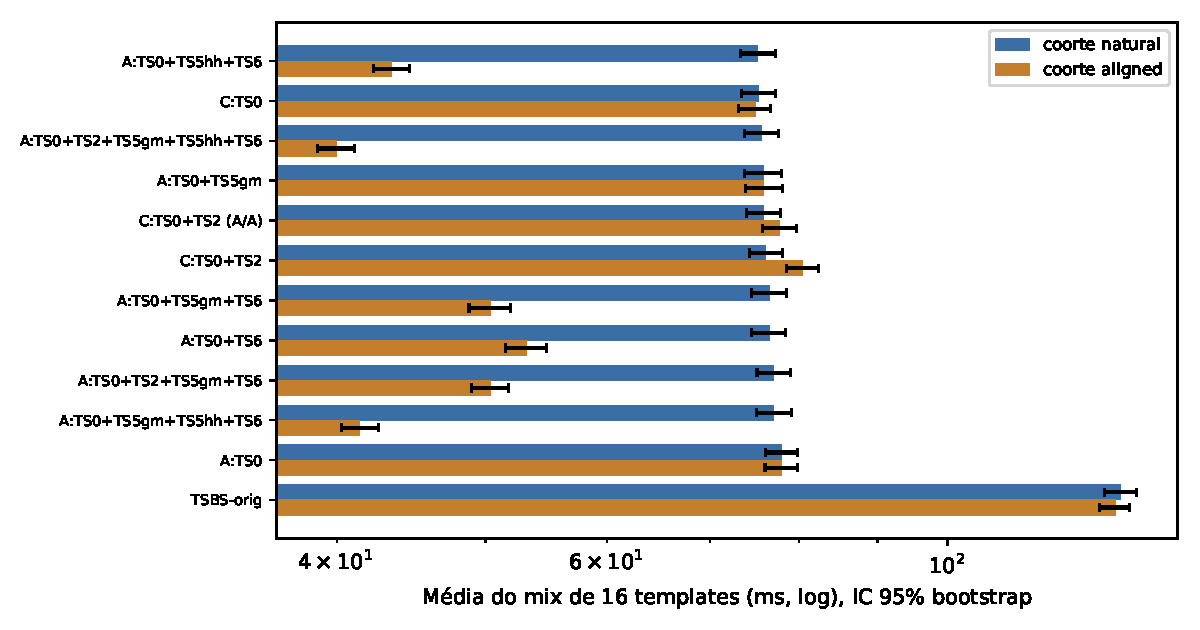
\includegraphics[width=0.95\linewidth]{figs/fig_v1_tsbs_mix.pdf}
\caption{Média do mix por coorte (escala log), IC 95\% bootstrap. ``C:'' perfil conservative; ``A:'' perfil conditional\_aligned.}
\end{figure}
\paragraph{Leitura.} Os dois perfis do Stage 8 correspondem a dois regimes reais. Com janelas arbitrárias (natural), as estruturas derivadas não são usadas e todos os deployments se comportam como TS0. Com janelas alinhadas, os rollups por hora e host (TS5hh, TS6) e o máximo global por minuto (TS5gm) cortam pela metade o custo das agregações. O custo dos rollups é de 1,1 a 1,6$\times$ o disco de TS0, e a carga sequencial praticamente não muda.


\subsection{Piso de ruído}
\begin{table}[H]\centering\small
\caption{Par A/A (mesmo deployment em keyspaces diferentes). Piso de ruído: natural \envnoiseN; aligned \envnoiseA.}
\begin{tabular}{@{}llccc@{}}\toprule Coorte & Par & Razão & IC 95\% & Piso\\\midrule
\tabin{tables/t_noise.tex}
\bottomrule\end{tabular}\end{table}

\subsection{Contrastes}
{\small\begin{longtable}{@{}lllccl@{}}
\caption{Contrastes pareados da média do mix (A/B).}\\
\toprule Coorte & A & B & A/B & IC 95\% & Veredito\\\midrule\endhead
\tabin{tables/t_contrasts.tex}
\bottomrule
\end{longtable}}

\subsection{Por template}
{\footnotesize\setlength{\tabcolsep}{3pt}
\begin{longtable}{@{}lrrrrrrc@{}}
\caption{Média por template (ms) nas coortes N e A: conservative rank 1, baseline TSBS e conditional rank 1. CQL: requisições do conservative rank 1.}\\
\toprule & \tabin{tables/perclass_head.tex} & \\
Template & N & A & N & A & N & A & CQL\\\midrule\endhead
\tabin{tables/t_perclass.tex}
\bottomrule
\end{longtable}}
\paragraph{Leitura.} As consultas pesadas (\texttt{cpu-max-all-32-24}, \texttt{double-groupby-*}, \texttt{high-cpu-all}, \texttt{lastpoint}) fazem de 200 a 400 requisições em TS0 (uma por host e métrica) e dominam a média do mix. No esquema original do TSBS, \texttt{lastpoint} lê a partição do dia inteira (693\,ms contra 86\,ms em TS0, que lê o último ponto com \texttt{LIMIT}), e \texttt{high-cpu-1} lê 10 partições em vez de uma. Parte da vantagem vem, portanto, do \emph{plano} de leitura por \texttt{(host, métrica)} com ordem descendente, um efeito análogo ao do Q8 no IoT-Benchmark.


\subsection{Avaliação do método}
\begin{table}[H]\centering\small
\caption{Preservação no conjunto medido (10 coberturas: HBench + Pareto não selecionados).}
\begin{tabularx}{\linewidth}{@{}lY@{}}\toprule
\tabin{tables/t_method.tex}
\bottomrule\end{tabularx}\end{table}
\paragraph{Leitura.} O regret é calculado no conjunto medido (10 coberturas); os 16 deployments dominados não foram medidos, o que é uma limitação. Na coorte aligned o escore ordena razoavelmente bem a leitura ($\tau=0{,}54$). Na natural ele não ordena ($\tau=-0{,}09$), porque todos empatam. Escolher só o menor escore ($k=1$) daria regret de 2,3\% na natural e 26\% na aligned. Os 7 escolhidos ao acaso entre os 10 medidos dariam 0,1\% e 1,5\%: o conjunto medido já é todo Pareto analítico, e por isso pouco discriminante.


\subsection{Ablações}
{\small\begin{longtable}{@{}p{3.4cm}rrcrrp{4.6cm}@{}}
\caption{Ablações: regra neutralizada e pipeline inteiro (Stages 1--8) regenerado. $|H|$ = tamanho do HBench; n/m = membros não medidos; $\le$ = limite superior do regret (só membros medidos).}\\
\toprule Ablação & $|H|$ & n/m & Mudou & Regret N & Regret A & Efeito\\\midrule\endhead
\tabin{tables/t_ablation.tex}
\bottomrule
\end{longtable}}
\paragraph{Leitura.} No TSBS o pipeline inteiro (Stages 1--8) é regenerado com a regra neutralizada, sem contratos rígidos de cardinalidade. As regras de rollup (TS5 e TS6) são as que sustentam o ganho na coorte aligned. Sem elas, o HBench resultante perde os deployments mais rápidos; alguns membros do HBench ablado não foram medidos, e por isso o regret aparece como limite superior. Na coorte natural nenhuma ablação piora o resultado, coerente com o empate geral.


\section{Hipóteses pré-registradas}
\begin{longtable}{@{}p{0.7cm}p{5.6cm}p{1.8cm}p{6.7cm}@{}}
\toprule & Hipótese & Resultado & Evidência\\\midrule\endhead
\tabin{tables/t_hyp.tex}
\bottomrule
\end{longtable}

\section{Aceitação}
\begin{minipage}[t]{0.5\linewidth}\centering\small
\begin{tabular}[t]{@{}lc@{}}\toprule Gate & \\\midrule
\tabin{tables/t_gates.tex}
\bottomrule\end{tabular}\end{minipage}\hfill
\begin{minipage}[t]{0.48\linewidth}\centering\small
\begin{tabular}[t]{@{}lc@{}}\toprule Teste negativo & \\\midrule
\tabin{tables/t_neg.tex}
\bottomrule\end{tabular}\end{minipage}

\medskip
Os gates foram recalculados a partir de \texttt{raw\_latencies.csv}: 32 classes $\times$ 12 variantes $\times$ 5 repetições $\times$ 12 rodadas, as 96 instâncias cobertas, 0 compactações durante as janelas e a razão máxima/mínima de posições de 1,47. Os hashes dos dados (arquivo do gerador e arquivo adaptado), das instâncias, do código e da fase de projeto não mudaram. \textbf{Status: ACEITO.}


\section{O que muda nas conclusões do TSBS}
\begin{enumerate}
\item \textbf{O TSBS deixa de ser o caso incompleto.} Agora tem execução completa do HBench, oráculo independente, dados do gerador oficial, armazenamento medido e a mesma estatística e o mesmo controle físico do IoT e do TPCx.
\item \textbf{Resultado principal.} O SchemaLens supera o esquema Cassandra original do TSBS por 1,7$\times$ na coorte natural e por até 3,2$\times$ na aligned. Parte do ganho vem do plano de leitura (\texttt{lastpoint}).
\item \textbf{Os perfis importam.} Os rollups só valem com janelas alinhadas; com janelas TSBS arbitrárias, um deployment só com TS0 é tão bom quanto qualquer outro. Escrever no artigo que o perfil \texttt{conditional\_aligned} depende de uma premissa de alinhamento que o gerador TSBS não garante.
\item \textbf{Achado de engenharia.} O gerador oficial no commit fixado emite \texttt{series\_bigint}; a premissa \texttt{series\_double} do Stage 9 só se sustentava com o fixture sintético.
\end{enumerate}


\section{Limitações}
\begin{itemize}
\item A escala é limitada pelo oráculo em memória (40 hosts, 36\,h, 600\,s), menor que o cenário analítico de 100 hosts, 60\,s e 3 dias usado na ativação.
\item As consultas vêm de \texttt{generate\_instances} (semântica dos templates TSBS) e são executadas pelo cliente Python; não houve replay dos bytes do \texttt{tsbs\_generate\_queries} nem do executor Go.
\item O regret é relativo às 10 coberturas medidas, e os 16 deployments dominados não foram medidos. Há 12 rodadas por repetição (desvio declarado).
\item A escrita é o carregador sequencial do Stage 6, sem manutenção incremental dos rollups.
\end{itemize}

\appendix
\section{Reprodução}
\begin{verbatim}
cd versao_ajustada/tsbs_tsdb
./gen_data.sh                   # gerador oficial TSBS (Go, commit fixado) em container golang
./run_all.sh smoke | freeze | measure | analyze | ablation | accept
../.venv/bin/python tsbs_v1/make_tables.py --run outputs/v1_run1
./run_all.sh report
\end{verbatim}
\end{document}
